\chapter[Influence of metallic artifacts during interictal epileptiform activity]{Influence of metallic artifact filtering on MEG signals for source localization during interictal epileptiform activity.}

\label{ch:4}
\textbf{Published as:} 
Migliorelli, C., Alonso J.F., Romero S., Ma\~nanas, Nowak R. and Russi A.
Influence of metallic artifact filtering on MEG signals for source localization during interictal epileptiform activity. \textit{Journal of Neural Engineering} 13(2):026029, 2016

doi:10.1088/1741-2560/13/2/026029

Impact Factor: 3.493; Position 10 of 76 (Q1) BIOMEDICAL ENGINEERING.

\textbf{Abstract:} \textit{Objective.} Medical intractable epilepsy is a common condition that affects 40\% of epileptic patients that generally have to undergo resective surgery. Magnetoencephalography (MEG) has been increasingly used to identify the epileptogenic foci through equivalent current dipole (ECD) modeling, one of the most accepted methods to obtain an accurate localization of interictal epileptiform discharges (IEDs). Modeling requires that MEG signals are adequately preprocessed to reduce interferences, a task that has been greatly improved by the use of blind source separation (BSS) methods. MEG recordings are highly sensitive to metallic interferences originated inside the head by implanted intracranial electrodes, dental prosthesis, etc and also coming from external sources such as pacemakers or vagal stimulators. To reduce these artifacts, a BSS-based fully automatic procedure was recently developed and validated, showing an effective reduction of metallic artifacts in simulated and real signals \citep{Migliorelli2015}. The main objective of this study was to evaluate its effects in the detection of IEDs and ECD modeling of patients with focal epilepsy and metallic interference. \textit{Approach.} A comparison between the resulting positions of ECDs was performed: without removing metallic interference; rejecting only channels with large metallic artifacts; and after BSS-based reduction. Measures of dispersion and distance of ECDs were defined to analyze the results. \textit{Main results.} The relationship between the artifact-to-signal ratio and ECD fitting showed that higher values of metallic interference produced highly scattered dipoles. Results revealed a significant reduction on dispersion using the BSS-based reduction procedure, yielding feasible locations of ECDs in contrast to the other two approaches. \textit{Significance.} The automatic BSS-based method can be applied to MEG datasets affected by metallic artifacts as a processing step to improve the localization of epileptic foci.

\textbf{Keywords:} magnetoencephalography, metallic artifact, automatic artifact reduction, blind source separation, epilepsy, IEDs

\section{Introduction}

Epilepsy is one of the most common neurological disorders affecting about one percent of the world population \citep{Ramey2013}. Its main therapeutic option relies on pharmacological treatment with antiepileptic drugs, which produce a seizure-free outcome for approximately 60\% of patients \citep{Schuele2008}. For the remaining 40\% of patients with focal refractory epilepsy, the most frequent therapeutic alternative is resective surgery of the epileptogenic area, which has demonstrated high rates of success \citep{Ramey2013}. 

An accurate localization of epileptic foci is necessary to minimize risk for surgical candidates. Frequently, invasive techniques such as subdural electrodes and depth electrodes are required to identify the epileptic focus. Over the last years, modern noninvasive whole-head systems based on magnetoencephalography (MEG) or electroencephalography (EEG) have been increasingly used to identify epileptogenic foci in children and adults requiring surgery \citep{Stufflebeam2009}. As a result of their high spatiotemporal resolution, MEG and EEG are able to track transient neural events that can be used to perform the source analysis which estimates the generators of electromagnetic activity inside the brain \citep{Gross2013}. Intracranial recordings are still the gold standard \citet{Panzica2013} for the epileptogenic zone identification, but even in this case, the evaluation with non-invasive techniques is crucial to determine the region where the electrodes will be implanted. For epilepsy studies, the identification of interictal epileptiform discharges (IEDs) is most commonly used for this purpose \citep{Bagic2011,Bouet2012}. The main advantage of MEG over EEG is that magnetic fields measured by MEG are much less influenced by the electrical conductivity of the tissues surrounding the cerebral cortex than electrical fields \citep{Shibasaki2007}. Both techniques can be considered complementary, and the detection of IEDs improves substantially when used simultaneously \citep{Lin2003,Pataraia2005,Knake2006}, although MEG has showed superior performance than EEG when localizing IEDs sources \citep{Amo2003,Stefan2004,Ramantani2006}

In clinical applications, one of the most accepted methods for obtaining an accurate localization of IEDs onset zone is the equivalent current dipole (ECD) model \citep{Anderson2014} that assumes that cortical activity captured by MEG signals is generated by a single dipolar source. This technique provides excellent clinical models whenever is reasonable to assume that the MEG field pattern arises from a single dipolar source \citep{Lutkenhoner1998}, as happens with focal epilepsy. Its accuracy for epileptic foci localization has been validated in several studies \citep{Stefan2003,Fischer2005,Oishi2006}.

Prior to ECD modeling of MEG or EEG data, signals must be adequately preprocessed to reduce biological and environmental interferences so that enough IEDs can be detected in spontaneous data \citep{Bagic2011}. After that, it is possible to adjust an equivalent dipole to cerebral activity reliably and with high goodness of fit and low confidence volume. Interferences may come from different sources such as cardiac, ocular, or muscular activity \citep{Stufflebeam2009}. Among the different possible methods of filtering, blind source separation (BSS) techniques have proven very effective for the reduction of many kinds of artifacts. Several studies have demonstrated the improvement of source localizations using BSS-based filtering approaches to remove cardiac, ocular or muscular artifacts \citep{Mantini2008,Fatima2013}. MEG recordings are also highly sensitive to metallic interferences originated inside the head, such as implanted intracranial electrodes, dental ferromagnetic prosthesis, and brackets; and also coming from external sources such as pacemakers, vagal stimulators \citep{Vrba2002} or deep brain stimulation \citep{Airaksinen2011}. Although an extremely magnetic hygiene inside the shielded recording room is required \citep{Hillebrand2013}, often it is not possible to eliminate all sources of metallic contamination and highly distorted data are then obtained. These artifacts appear modulated by breathing and cardiac rhythms and affect the whole record, overlapping the brain activity. In addition, there are usually a number of channels, grouped in one or more areas of the scalp, with a very high level of contamination and whose cerebral activity is masked almost completely \citep{Migliorelli2015}.

Modeling ECDs from IEDs with such metallic artifacts is not always possible due to the high distortion of the data. Worse still, patients whose recordings are highly affected by this interference have to be excluded from analysis. If not excluded, a reliable dipole localization can only be achieved by selecting subsets of channels associated with the dipolar field and rejecting those with high metallic interference \citep{Bagic2011}. However, this reduction of the number of channels close to the epileptic region has several disadvantages: firstly, an inappropriate channel selection can lead to an incorrect source estimation due to the loss of valuable information \citep{Bagic2011}; secondly, removing the most artifacted channels does not necessarily mean that metallic interference has been cleaned, since it can also be present in the rest of the record; and thirdly, if high levels of metallic artifacts are present, IEDs may stay masked behind them, rendering visual identification very difficult or impossible at all. To overcome these limitations, a fully automatic procedure for reducing metallic interference from spontaneous MEG signals based on BSS recently showed an effective reduction of metallic artifacts in simulated and real signals \citep{Migliorelli2015}.

Signal space separation and temporal signal space separation (tSSS) algorithms \citep{Taulu2006} have proven its efficiency removing MEG artifacts in several studies \citep{Song2009,Kakisaka2012,Jin2013,Wang2013}. However, these algorithms are only available, specifically designed and mandatory for Elekta-Neuromag systems \citep{GonzalezMoreno2014}. On the other hand, the filtering approach presented in \citep{Migliorelli2015} is based on standard libraries which are freely available and can be used with signals from different MEG systems such as CTF/VSM, 4D Neuroimaging, Elekta and Yokogawa.

The main objective of the present study was to evaluate the effects of this automatic filtering procedure in the detection of IEDs and EDC modeling of patients with focal epilepsy and metallic interference, assessing the hypothesized improvement due to metallic artifact reduction. A comparative study of the resulting positions of ECDs was performed for three cases: considering the acquired data without removing metallic interference; rejecting only channels with large metallic artifacts; and after BSS-based reduction of metallic artifacts. To analyze the results obtained for each situation, measures of dispersion and distance of EDCs were defined.

\section{Materials and methods}

\subsection{Patients, acquisition settings and previous preprocessing}

14 patients diagnosed with intractable epilepsy (age 15.34 $\pm$ 10.66 years, mean and standard deviation) were selected for this study. All of them had some kind of nonremovable device that produced metallic interferences: eight patients had dental orthodontics, four an implanted subdural grid, one a vagus nerve stimulator, and one ventricular bypass valve. All patients selected for this study presented interictal activity coming from one focal generator. Table \ref{tb:2-1} show the summary of the data of all 14 subjects.

\begin{table}[h!]
\centering
\caption{Summary of all patients. Age, type of epilepsy, type of metallic artifacts.}
\small
\vspace{3mm}
\label{tb:2-1}
\begin{threeparttable}
\begin{tabular}{rrrl}
Subject       & Age            & Type of epilepsy & Type of metallic artifacts \\ \hline
              &                &                  &                            \\
1             & 10             & PLE              & Dental                     \\
2             & 34             & TLE              & Dental                     \\
3             & 31             & TLE              & Dental                     \\
4             & 25             & TLE              & Vagus nerve stimulator     \\
5             & 19             & PLE              & Subdural implant           \\
6             & 15             & TLE              & Subdural implant           \\
7             & 4              & TLE              & Ventricular bypass valve   \\
8             & 16             & FLE              & Subdural implant           \\
9             & 25             & PLE              & Dental                     \\
10            & 8              & TLE              & Dental                     \\
11            & 9              & FLE              & Dental                     \\
12            & 5              & TLE              & Subdural implant           \\
13            & 6              & TLE              & Dental                     \\
14            & 3              & TLE              & Dental                     \\
\textbf{Mean} & \textbf{15.38} &                  &                            \\
\textbf{Std}  & \textbf{10.66} &                  &                           
\end{tabular}
\begin{tablenotes}
      \small
      \item \begin{flushright} TLE: temporal lobe epilepsy, PLE: parietal lobe epilepsy, FLE: frontal lobe epilepsy.
     \end{flushright}
    \end{tablenotes}
    \end{threeparttable}
\end{table}

MEG signals were acquired in a magnetically shielded room during 10 min with eyes closed using a whole-head 148-channel magnetometer system (4D-Neuroimaging/BTi, San Diego, California, USA) and sampled at 678.19 Hz (bandwidth DC to 250 Hz). A 19-channel EEG was simultaneously recorded using a Neurofax amplifier (Nihon-Kohden Co., Tokyo, Japan), with sampling rate set to 512 Hz (bandwidth 3–70 Hz). The relative position of the patient's head with respect to the MEG sensors was recorded continuously using head-localization coils.

Signals were imported into MATLAB using the Fieldtrip toolbox \citep{Oostenveld2011} and processed with an 8th order bandpass Butterworth filter with cutoff frequencies set to 3 and 70 Hz as recommended by the clinical practice guidelines \citep{Bagic2011}.

\subsection{Volume conduction model} \label{sec:VCM}

The patient's index points and head shape were digitized with a 3Space Fasttrack (Polhemus, Vermont, USA) prior to each measurement. The nasion, an anatomical landmark, and the left and right ear canal points served as index points and were used to define a right-handed coordinate system, called headframe coordinate system: the \textit{x}-axis points to the front, the \textit{y}-axis to the left, and the \textit{z}-axis to the top of the head.

The scalp and brain meshes for each subject were obtained by aligning and warping the default anatomy provided by the Montreal Neurological institute with Brainstorm software \citep{Tadel2011}. The volume conduction model was obtained with the localspheres algorithm provided by Fieldtrip in which a local sphere is fitted to the brain surface for each separated channel \citep{Huang1999}.

\subsection{IED identification}

MEG data was visually inspected by three different experts for detection of IEDs. Well-defined IEDs, were selected following the definition of basic morphologic IED characteristics \citep{Nowak2009,Jaseja2012}. Inspection of the whole-head MEG data took into account the simultaneous EEG recordings to verify IED presence and discard other waveforms, especially in highly artifacted MEG signals. For each IED identified by the three experts, the corresponding magnetic and electric isofield maps were obtained and inspected to assess its spatial distribution, looking for dipolar patterns on a sample-by-sample basis. Only those IEDs that produced stable voltage fields in the simultaneous EEG showing little change in shape and position over time where used since these are the most appropriate IEDs to be modeled by a dipolar distribution \citep{Townsend2008}. The onset of a spike was defined as the time point when spiking activity was distinguishable from the background noise and when a single distinctive dipolar pattern was observed in the simultaneous EEG (figure \ref{fig:2-1}). The peak of a spike was defined as the maximum peak value after the spike onset. The channel closest to the origin of the dipolar activity was defined as the central channel. Since only a small number of MEG sensors show a prominent signal for a single source \citep{Hamalainen1993}, a subset of 36 neighboring channels (25\% of the total number of channels) at the time interval under study were selected for further ECD calculations. This selection was done in order to prevent under- and over-fitting phenomena as it has been demonstrated that not much is gained when using more than 40 channels when modeling spike potentials \citep{Ebersole2003}.

\begin{figure}[h]
\centering
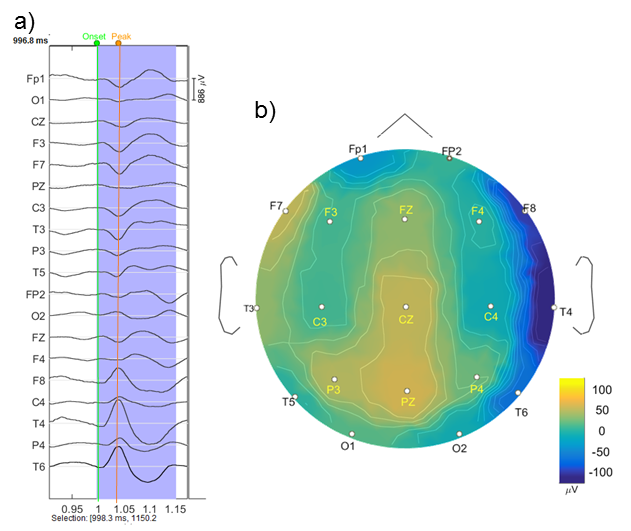
\includegraphics[width=1\textwidth]{Images/fig2-1.png}
\caption{(a) Example of IED identification for subject 1 by in EEG simultaneous data. Green line denotes the spike onset and orange line the spike peaks. (b) Topographical map at spike onset where a dipolar distribution between T4 and P4 is observed.}
\label{fig:2-1}
\end{figure} 

\subsection{Artifact removal}

In this study, two different strategies were used to remove interference coming from metallic sources. The first consisted in the rejection of highly artifacted channels, and the second involved the application of a BSS-based automatic procedure for metallic artifact reduction.

Regarding channel rejection, the most affected channels were easily identified by visual inspection, because these prominent metallic artifacts exhibit characteristic features: high amplitude in comparison with the remaining MEG leads; and slow and regular waveforms, usually modulated by cardiac and respiratory activity \citep{Hillebrand2013}. The three experts examined the 37 channels selected for each IED and visually identified the artifacted channels following these criteria. Those channels identified by the three experts were excluded from the subsequent ECD estimation. Moreover, in order to prevent the over-fitting of the dipole model due to the channel reduction, additional and nearby artifact-free channels were selected to replace the artifactual channels in the ECD estimation. Thus, this ECD estimation was always performed using 37 channels. With respect to automatic artifact reduction, the 10 min MEG recordings of each patient were filtered of metallic contamination by using the fully automatic procedure described in \citep{Migliorelli2015}. This method is based on the AMUSE algorithm and decomposes the signals into independent components exploiting second order statistics \citep{Tong1991}, which proved effective enough in the separation of components corresponding to various types of artifacts \citep{Escudero2010}. The employed automatic methodology decomposed MEG signals into as many independent components as available channels, and these components were checked for known metallic interference features: regular behavior, measured by the sample entropy; and low frequency content, measured by the percentage of energy below a specific frequency. Given these characteristics of each independent component, a two-step process was carried out, firstly to define the area or areas of the scalp corresponding to artifacted regions, and secondly to detect all independent components related to metallic activity. After these steps, the corrected artifact-free MEG data was obtained by reconstruction without considering the independent components associated with metallic artifacts. This method for automatic artifact reduction applied was previously validated with real and simulated signals in the study published in \citep{Migliorelli2015}. The amount of error for the artifact reduction procedure was significantly reduced (worst case around 2.5\%). A detailed description of the actual algorithm is given in \citep{Migliorelli2015}.

To quantify the amount of interference removed, an artifact-to-signal ratio (ASR) was defined for each IED:

\begin{equation} \label{eq:2-1}
ASR = 100 \cdot \sum_{n} \langle \frac{\sum_{t}^{T} (s_{n}(t)-sf_{n}(t))^2}{\sum_{t}^T sf_{n}(t)} \rangle ,
\end{equation}

where $n$ denotes the MEG channel, $sf$ represents the filtered signal, $s$ is the original raw signal, and $ \langle \rangle $ indicates average over all samples comprised between the beginning and the end of the IED \citep{Nowak2009}.

\subsection{Estimation of the ECD}

Single dipole fitting was performed by means of the FieldTrip toolbox \citep{Oostenveld2011}, which uses grid search and nonlinear fitting trying to explain the MEG topography under study. The ECD model was fitted to the patient's head volume conduction model obtained as explained in section \ref{sec:VCM}. No averaging of IEDs was performed, and a set of dipoles were estimated for each IED during its whole rising phase: from its onset to the spike peak using 4.5 ms time steps (i.e. three samples for each dipole). Each ECD was computed using the data of the subset of channels selected previously. The model was calculated using the maximum likelihood estimation approach that improves the accuracy of the dipole source localization \citep{Lutkenhoner1998}. The baseline noise (50 ms of recording not containing brain activity of interest) was considered as a multivariate Gaussian distribution and characterized by a covariance matrix.

The performance of the fitting procedure was assessed by means of the following goodness-of-fit measure:

\begin{equation} \label{eq:2-2},
gof = 100 \cdot ( 1 - \frac{(\upsilon - \hat{\upsilon})^T ((\upsilon - \hat{\upsilon})}{\upsilon ^{T} \upsilon}),
\end{equation}

where $\upsilon$ and $\hat{\upsilon}$ represent the vectors of the measured and modeled magnetic fields, respectively and by the 95\% confidence volume defined as the volume of the ellipsoid comprising the confidence intervals of each of the dipole projections: $x$, $y$ and $z$:

\begin{equation} \label{eq:2-3}
V = \frac{4\pi}{3} \cdot \frac{CI_x}{2} \cdot \frac{CI_y}{2} \cdot \frac{CI_z}{2}, 
\end{equation}

where $CI_x$, $CI_y$ and $CI_z$ represent the 95\% confidence interval in each of the dipole directions. 

Dipole fitting was applied to all IEDs and their corresponding 37 selected channels for three different conditions: (1) using all channels without removing metallic interference; (2) rejecting channels with large metallic artifacts visually determined by the experts; and (3) after applying the BSS-based metallic reduction procedure. Ten IEDs were selected for further study, corresponding to those which obtained the lowest confidence volume in the first condition, with a minimum gof threshold value of 85\%.

\subsection{Evaluation of estimated sources}

To evaluate the differences among the three conditions, the distribution of the obtained dipoles at the onset time for each patient was analyzed by means of its central position and dispersion. Additionally, the running distance of the path followed by dipoles associated to each IED was computed. For these purposes, IEDs showing estimated sources outside of the head were excluded to maintain anatomical plausibility. To calculate this running distance, the whole computed ECDs from the spike onset to the spike peak were used to check the consistency of each IED during the rising phase of the spike.

The distance of each IED path was computed as the sum of the distances between consecutive dipoles. Since IEDs that produce a stable magnetic field and show little change in shape and position over time where used in this study, it is expected to find a slight unidirectional change in the dipole position during the whole rising phase of the dipole \citep{Townsend2008}(Townsend and Ebersole 2008). Moving dipole models that make sudden changes in direction may be the result of multiple sources overlapping, as occurs when dealing with metallic artifact. For this reason, distance values are expected to be lower when the source is produced by a single dipolar source.

The central source position was obtained as the averaged position of all estimated ECDs of the ten selected IEDs of each patient. The total dispersion was calculated as the average distance between each ECD and the central position.

\section{Results}

\subsection{Artifact removal}

For the channel rejection approach, the 37 selected channels of each selected IED and patient were visually inspected by the three experts. Channels with presence of metallic artifacts showing regular behavior and considerably higher amplitudes than the rest of the channels were removed from the analysis, but only if they had been identified by the three experts. The agreement among experts was quantified by calculating the kappa index \citep{Viera2005} and a high inter-rater reliability was obtained (kappa = 0.87 $\pm$ 0.10). Table \ref{tb:2-2} contains the number of rejected channels and shows that four subjects did  not show artifacted channels in the area of the dipole. No rejection was performed in these cases.

\begin{table}[!h]
\setlength{\tabcolsep}{4pt}
\centering
\caption{Results for all patients}
\small
\vspace{3mm}
\hspace*{-0.2cm}
\label{tb:2-2}
\begin{threeparttable}
\begin{tabular}{rrrrrrrrrrrrrrr}
Subj. & R.chan. & R.IC & ASR     & R.IEDs & \multicolumn{3}{c}{\begin{tabular}[c]{@{}c@{}}Confidence\\ Volume\end{tabular}} & \multicolumn{3}{l}{Dispersion} & \multicolumn{3}{l}{Distance} \\ \hline
      &                                                    &       &         &                                   &                                   &                           &                          &                          &          &          &          &          &          &        \\
      &                                                    &       &         & NC                                & CR                                & NC                        & CR                       & AF                       & NC       & CR       & AF       & NC       & CR       & AF     \\
1     & 7                                                  & 10    & 549.75  & 1                                 & 1                                 & 65.65                     & 48.24                    & 24.97                    & 1.86     & 1.18     & 0.62     & 4.15     & 3.62     & 2.19   \\
2     & 2                                                  & 6     & 93      & 1                                 & 0                                 & 39.47                     & 31.55                    & 10.85                    & 3.31     & 2.22     & 2.16     & 7.93     & 18.49    & 4.21   \\
3     & 1                                                  & 15    & 54.57   & 1                                 & 1                                 & 49.14                     & 19.24                    & 4.61                     & 2.97     & 2.92     & 3.05     & 16.18    & 10.74    & 5.50   \\
4     & 0                                                  & 21    & 1147.72 & 2                                 & 2                                 & 18.91                     & 18.91                    & 3.35                     & 3.88     & 3.88     & 0.95     & 11.88    & 11.88    & 2.83   \\
5     & 0                                                  & 17    & 92.23   & 0                                 & 0                                 & 15.51                     & 15.51                    & 14.14                    & 1.12     & 1.12     & 1.01     & 3.79     & 3.79     & 2.12   \\
6     & 12                                                 & 36    & 1991.77 & 2                                 & 1                                 & 67.84                     & 35.28                    & 18.87                    & 7.30     & 3.54     & 1.92     & 5.65     & 6.98     & 2.78   \\
7     & 3                                                  & 7     & 283.58  & 5                                 & 1                                 & 27.55                     & 27.77                    & 24.88                    & 3.12     & 1.94     & 1.98     & 8.01     & 5.55     & 3.13   \\
8     & 0                                                  & 14    & 195.6   & 1                                 & 1                                 & 47.94                     & 47.94                    & 37.51                    & 2.44     & 2.44     & 2.21     & 23.84    & 23.84    & 2.27   \\
9     & 0                                                  & 4     & 66.7    & 1                                 & 1                                 & 32.04                     & 32.04                    & 11.85                    & 1.65     & 1.65     & 1.54     & 14.60    & 14.60    & 3.05   \\
10    & 4                                                  & 8     & 1241.27 & 2                                 & 2                                 & 26.24                     & 19.58                    & 15.13                    & 8.03     & 3.15     & 1.08     & 10.83    & 6.21     & 3.41   \\
11    & 4                                                  & 11    & 145.42  & 0                                 & 0                                 & 27.24                     & 21.29                    & 21.19                    & 1.14     & 0.77     & 0.76     & 1.52     & 1.74     & 1.86   \\
12    & 4                                                  & 18    & 170.57  & 1                                 & 1                                 & 79.56                     & 12.50                    & 8.84                     & 1.37     & 1.03     & 1.12     & 5.12     & 5.39     & 3.32   \\
13    & 7                                                  & 6     & 939.85  & 5                                 & 1                                 & 14.11                     & 8.76                     & 7.78                     & 7.10     & 3.65     & 3.12     & 13.06    & 3.07     & 2.49   \\
14    & 5                                                  & 3     & 733.14  & 1                                 & 0                                 & 9.50                      & 9.45                     & 8.84                     & 2.42     & 1.64     & 0.51     & 6.91     & 4.44     & 1.82   \\
      &                                                    &       &         &                                   &                                   &                           &                          &                          &          &          &          &          &          &        \\
Mean  & 3.23                                               & 12.57 & 550.37  &                                   &                                   & 37.19                     & 24.72                    & 15.20                    & 3.41     & 2.22     & 1.57     & 9.53     & 8.6      & 2.93   \\
Std   & 3.48                                               & 8.72  & 588.41  &                                   &                                   & 21.17                     & 12.80                    & 9.43                     & 2.36     & 1.06     & 0.85     & 5.99     & 6.52     & 1.00  
\end{tabular}
\begin{tablenotes}
      \small
      \item \begin{flushright} R.Chan: Removed Channels, R.IC: Removed independent components R.IEDs: Removed IEDs, NC: Non corrected, CR: Channel removal, AF: Artifact filtering
     \end{flushright}
    \end{tablenotes}
    \end{threeparttable}
\end{table}


Figure \ref{fig:2-2}(a) shows, as an example, a 5 s epoch of the 37 selected raw channels used to fit ECDs in the case of metallic artifacts of dental origin affecting the right temporal zone of the scalp (patient 1). Highly artifacted channels selected to be removed are emphasized in red.

The BSS-based automatic artifact reduction procedure was applied to the 10 min records and independent components corresponding to metallic artifacts were removed before signal reconstruction. Figure \ref{fig:2-2}(b) shows an example of the corrected MEG signals, where it can be observed how the energy of highly artifacted channels decreased markedly. The number of independent components removed was 12.57 $\pm$ 8.72 (out of 148, mean and standard deviation for all patients).

\begin{figure}[h]
\centering
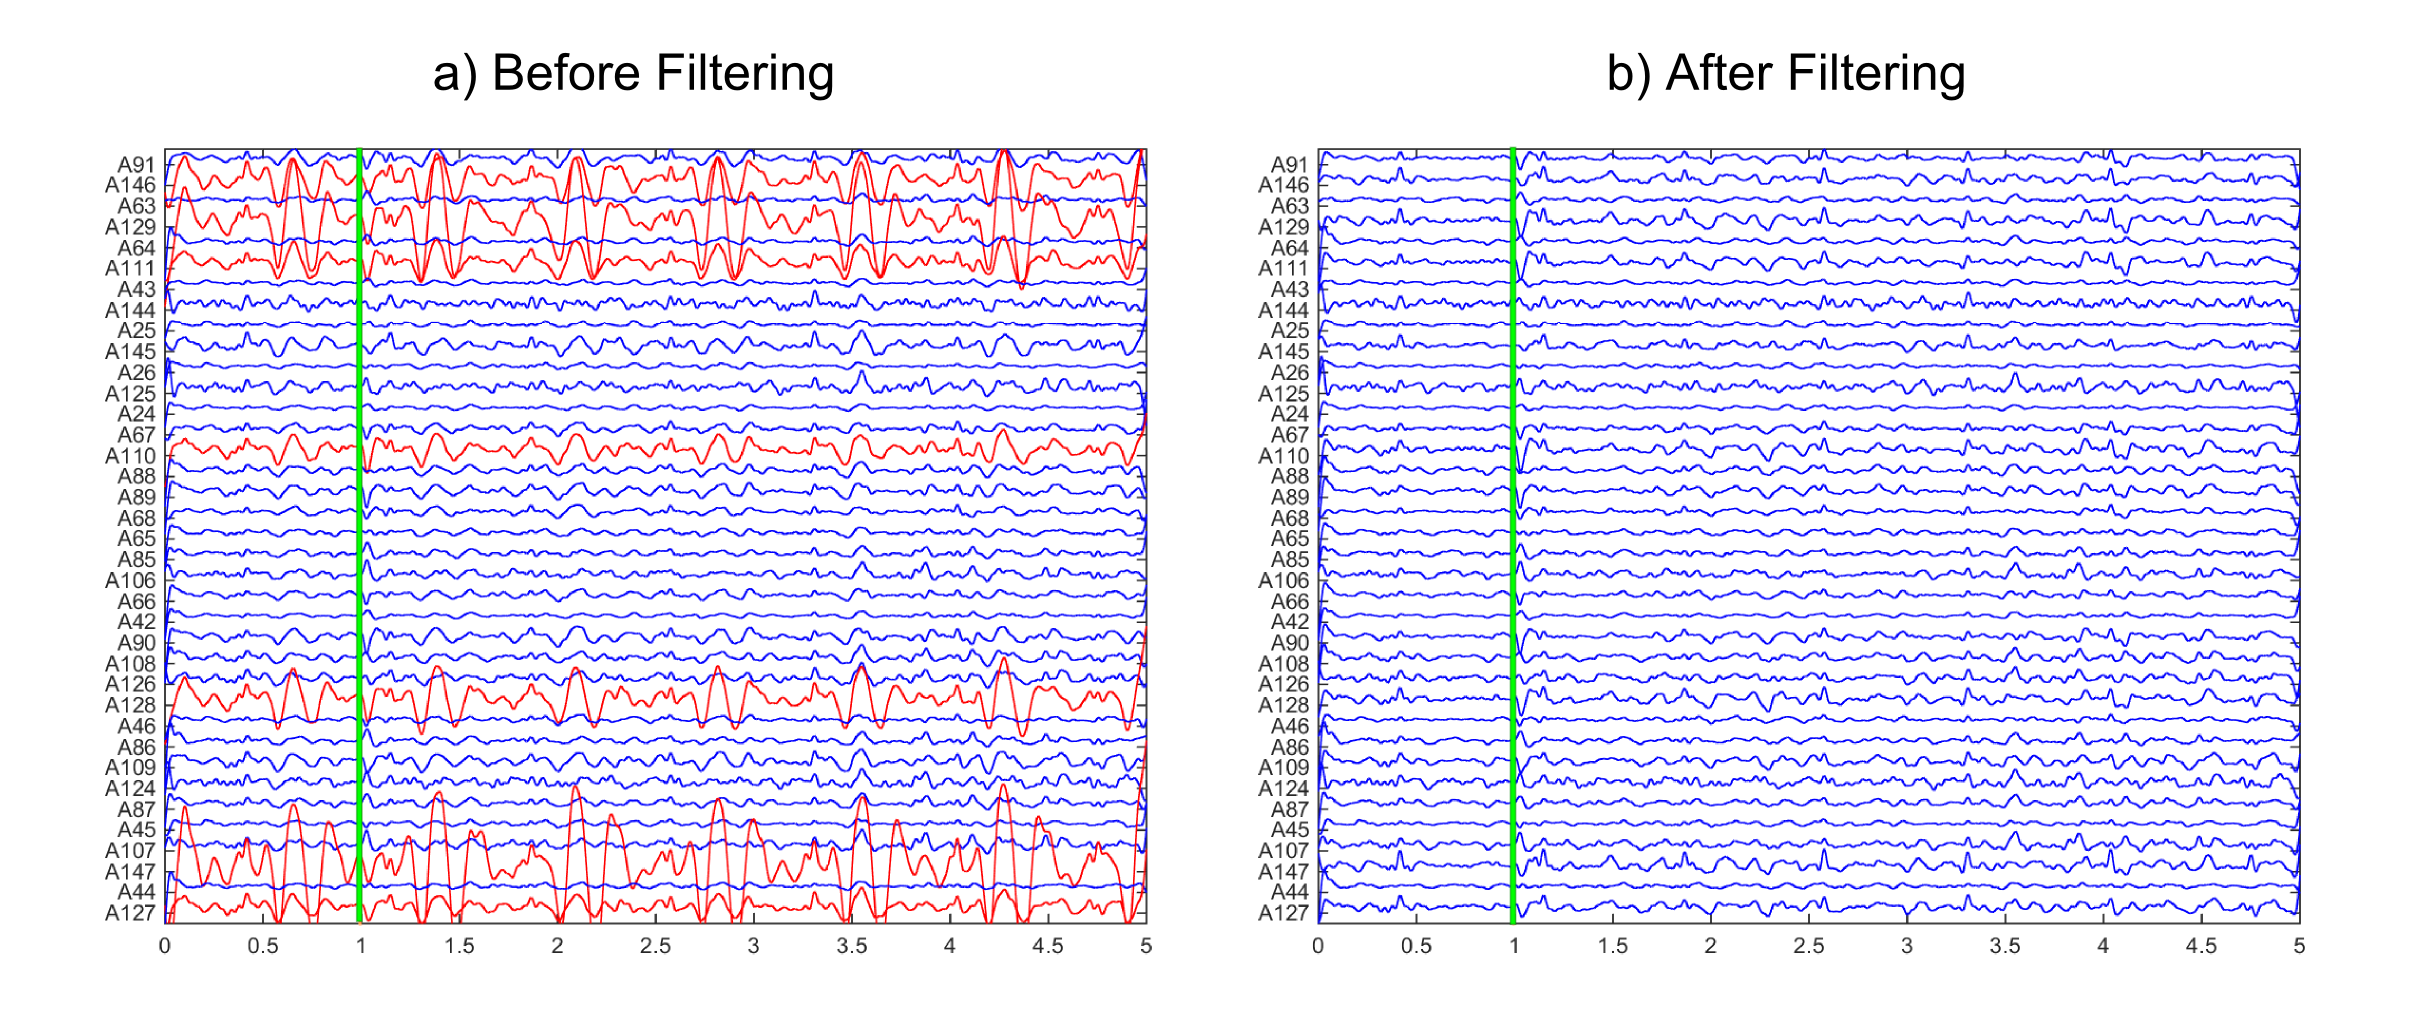
\includegraphics[width=1\textwidth]{Images/fig2-2.png}
\caption{5 s epoch corresponding to 37 MEG channels for subject 1 selected for dipole fitting. Vertical lines show the onset of at the same well-defined IED shown in figure \ref{fig:2-1}. (a) RAW signal before applying automatic reduction procedure. Red channels were selected by experts as highly artifacted channels and removed in the channel rejection procedure. (b) Corrected MEG signals obtained after applying automatic AMUSE-based metallic removal procedure.}
\label{fig:2-2}
\end{figure} 

The topographic distribution of normalized energy corresponding to the removed metallic activity is shown in the maps of figure \ref{fig:2-3}. Each map presents a different distribution of energy that mainly depended on the type of metallic artifact. Table \ref{tb:2-2} also shows the average ASR obtained for each patient, evidencing a high variability among subjects probably due to the different nature of metallic contamination.

\begin{figure}[h]
\centering
\hspace*{-0.75cm}
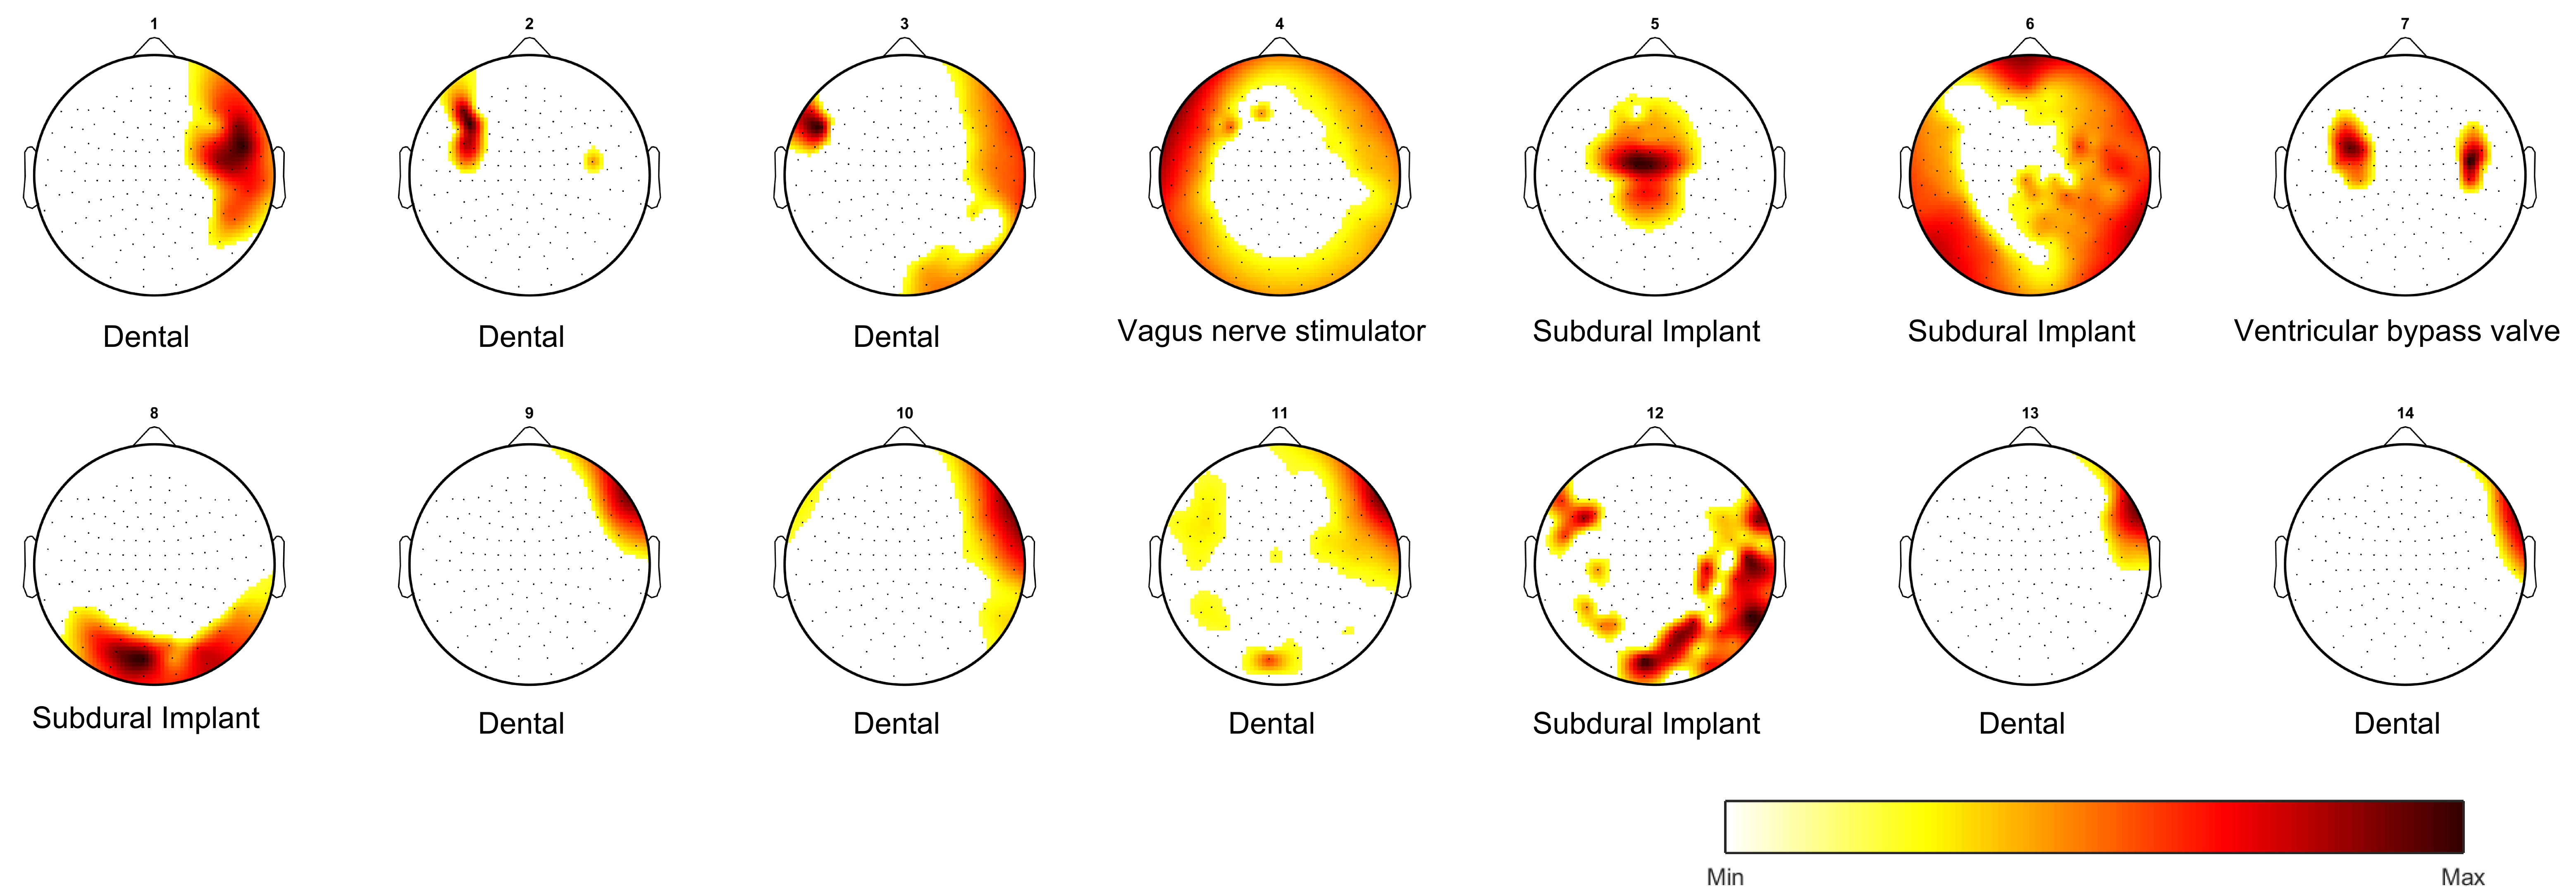
\includegraphics[width=1.1\textwidth]{Images/fig2-3.png}
\caption{Topographic distribution of normalized energy corresponding to the removed metallic activity for the 14 subjects. Artifact distribution of energy mainly depended on the type of metallic interference, to its position and size.}
\label{fig:2-3}
\end{figure} 


\subsection{ECD estimation}

Temporal signals and electric isofields from each IED were analyzed to identify spike onsets time considering morphological IED characteristics and field dipolar distribution (figure \ref{fig:2-1}). Figure \ref{fig:2-4}(a) shows the magnetic isofield of a spike, corresponding to the spike in figures \ref{fig:2-1} and \ref{fig:2-2} (onset indicated by a green vertical line), before applying the artifact reduction procedure. Figures \ref{fig:2-4}(b) and (c) show the equivalent maps to figure \ref{fig:2-4}(a) when channel rejection and the automatic artifact reduction were performed, respectively. Magnetic isofields changed, suggesting different dipole locations depending on the approach. Figure \ref{fig:2-4}(c) presented a more plausible dipolar distribution more similar to EEG distribution (figure \ref{fig:2-1}(b)).

\begin{figure}[h]
\centering
\hspace*{-1cm}
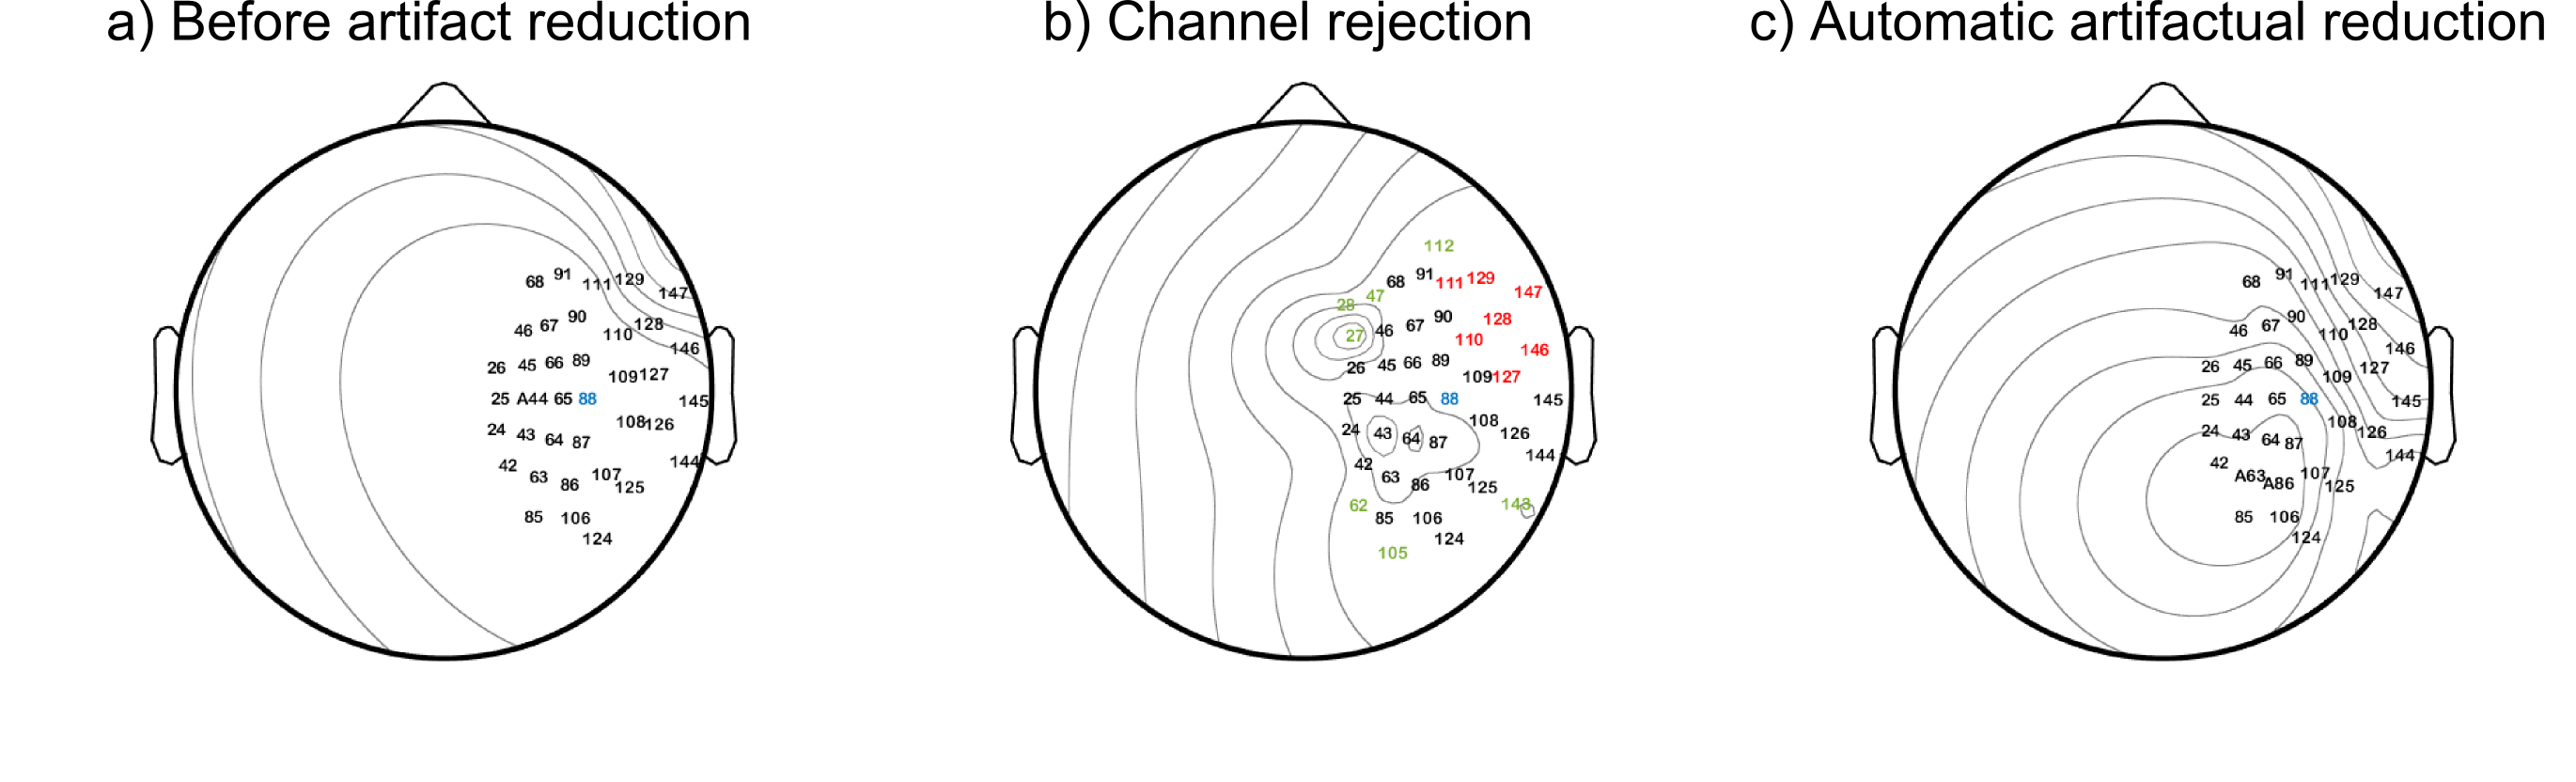
\includegraphics[width=1.1\textwidth]{Images/fig2-4.png}
\caption{Magnetic isofields computed for the 37 selected channels corresponding to the same IED onset shown in figure \ref{fig:2-1}. For the three approaches: (a) before applying any filtering procedure (no correction), (b) after channel rejection, (red channels were removed, green channels were included); and (c) after applying the metallic reduction procedure. The central channel is shown in blue.}
\label{fig:2-4}
\end{figure} 

Dipoles were calculated at each IED onset in three cases: (1) using all 37 selected channels without any kind of correction; (2) rejecting channels with clearly visible metallic artifacts; and (3) applying an automatic BSS-based artifact reduction. The ten IEDs whose dipoles achieved the lowest \textit{V} in the first case were selected for further study, taking into account a minimum \textit{gof} value of 85\%. Paired sample T-tests with significance set to 0.05 were used to compare the three approaches. The confidence volume measure showed significant differences between the three approaches (\textit{p-value} $<$ 0.04 in any case). No statistically significant differences were obtained for the \textit{gof} values.

Figure \ref{fig:2-5} shows the positions of the dipoles obtained for the ten IEDs of patient 1 (planes \textit{XY}, \textit{XZ}, and \textit{YZ}). Dipoles are drawn inside the anatomical representation of the head and brain of the patient. Dipoles that appeared outside of the brain cortex (see dipole 4 of the no-correction approach, in blue), were discarded for subsequent measurements of dispersion and distance, which were calculated for all 14 subjects and the three approaches.

\begin{figure}[h]

\centering
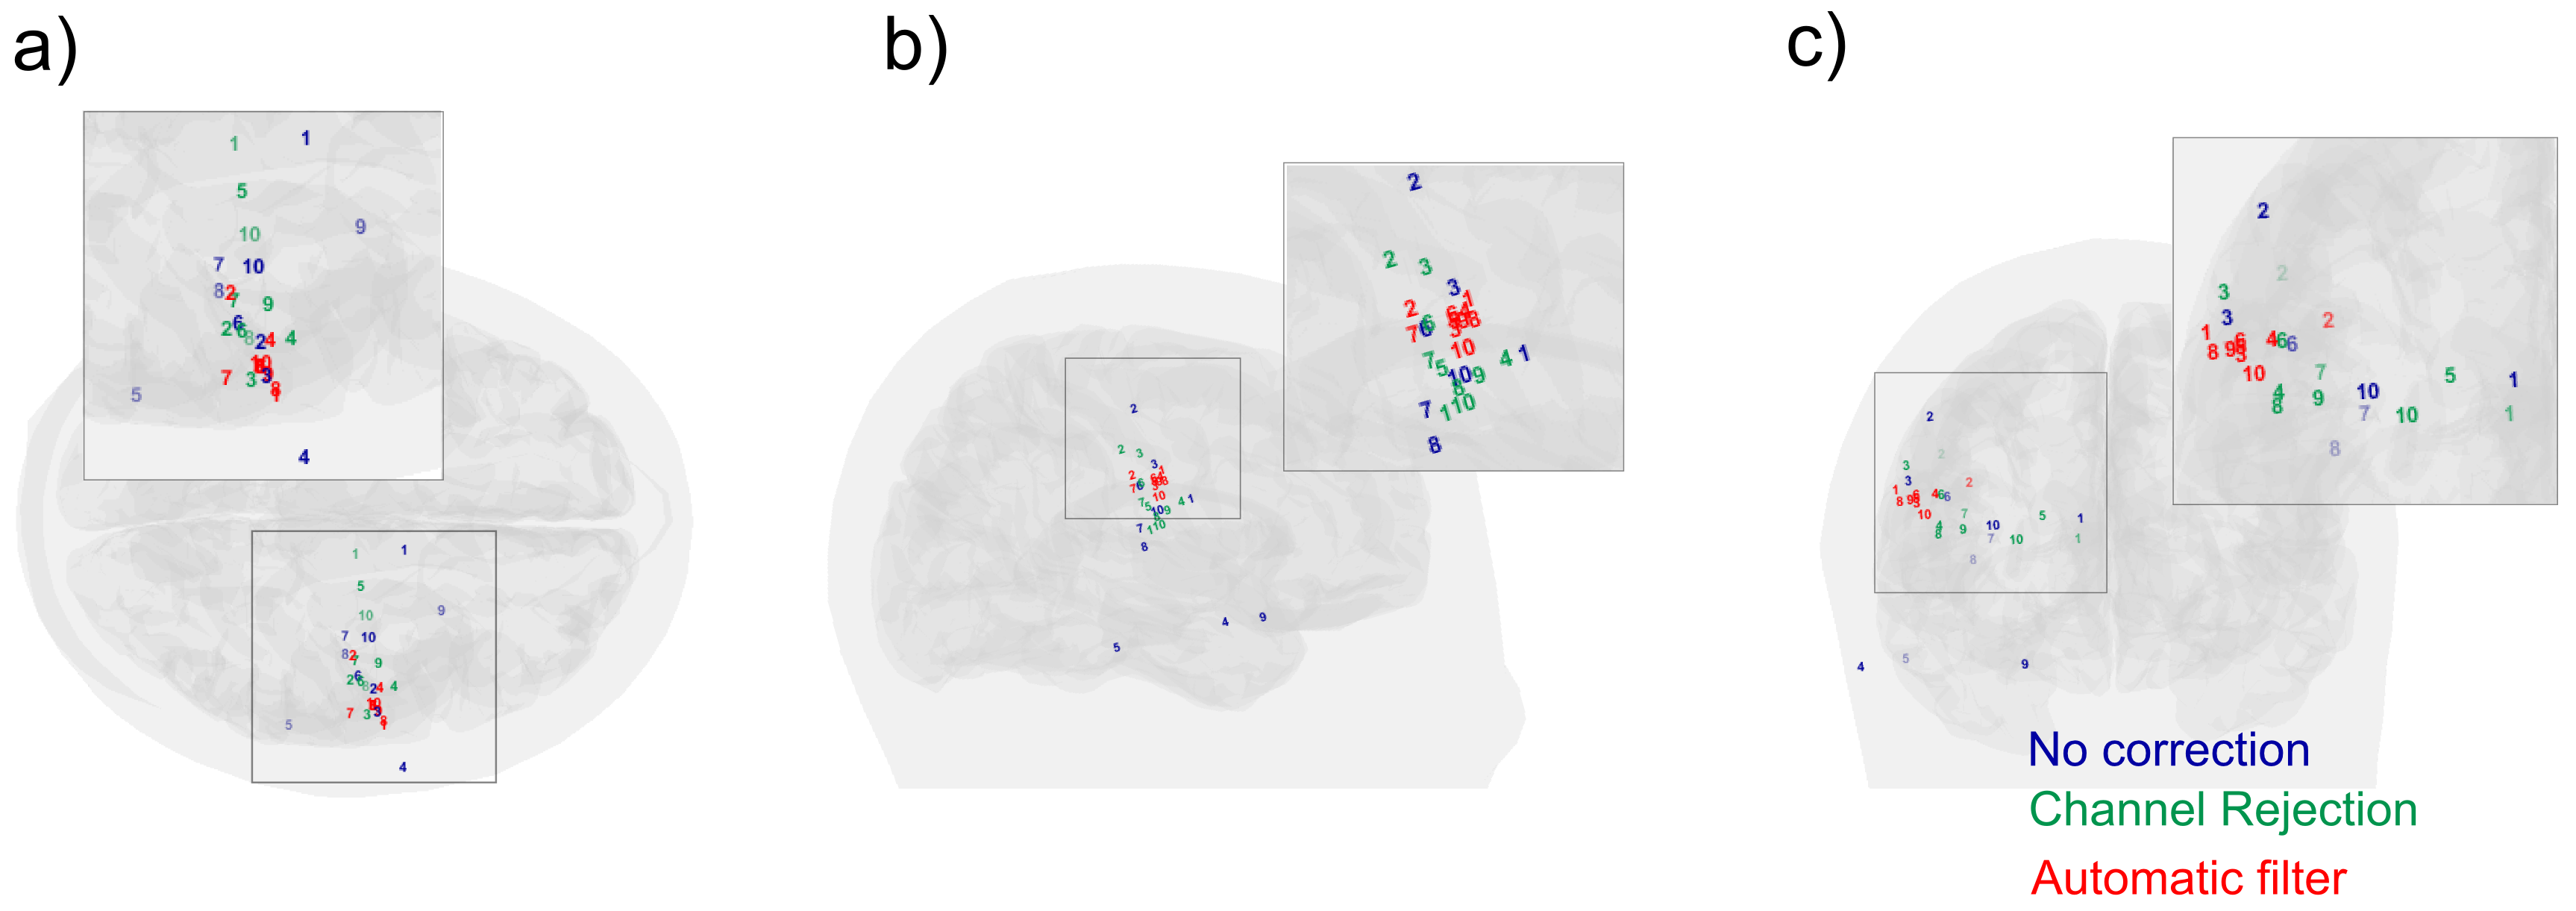
\includegraphics[width=1\textwidth]{Images/fig2-5.png}
\caption{Dipoles obtained for the ten IEDs of Patient 1 (a) \textit{XY} plane, (b) \textit{XZ} plane and (c) \textit{YZ} plane. Blue, green and red dipoles belong to no-correction, channel rejection and automatic filter procedures. Dipole 4, located outside the brain in the no-correction procedure, was discarded for the subsequent measurements of dispersion and distance.}
\label{fig:2-5}
\end{figure} 

Table \ref{tb:2-2} shows the obtained dispersion values for each patient and the number of spikes discarded due to their location outside the brain. Interestingly, all dipoles obtained after BSS-based artifact reduction were found inside the head, and therefore it was possible to use all of them to estimate the dispersion measure. The average dispersion for all patients was of 3.41 $\pm$ 2.36 cm if no artifact filtering was applied, and this value decreased to 2.22 $\pm$ 1.06 cm when channel rejection was performed (\textit{p-value} = 0.06 with respect to no artifact correction), and decreased even more if automatic BSS-based reduction was chosen, reaching a value of 1.57 $\pm$ 0.85 cm (\textit{p-values} of 0.007 and 0.036 with respect to no artifact correction and channel rejection approaches, respectively). Differences between automatic approach and the two previous were statistically significant (paired T-tests, significance set to 0.05), with probability values of 0.007 and 0.036 for non-corrected signals and channel rejection approaches, respectively.

With respect to the running distance of ECDs, figure \ref{fig:2-6} shows an example of the positions obtained for the consecutive dipoles fitted during the rising phase of an IED. Table \ref{tb:2-2} demonstrates that the distance traveled by ECDs was clearly lower after applying the automatic procedure: distances for the naive and the channel rejection approaches showed similar values of 9.53 $\pm$ 5.99 cm and 8.60 $\pm$ 6.52 cm, respectively (no significant differences were found, \textit{p-value} = 0.277), whereas the automatic filtering obtained a measure of 2.93 $\pm$ 1.00 cm. Analogously to the dispersion measure, differences between the automatic approach were significant, with probability values of 0.001 and 0.003 for non-corrected signals and channel rejection approaches, respectively.

\begin{figure}[h]
\centering
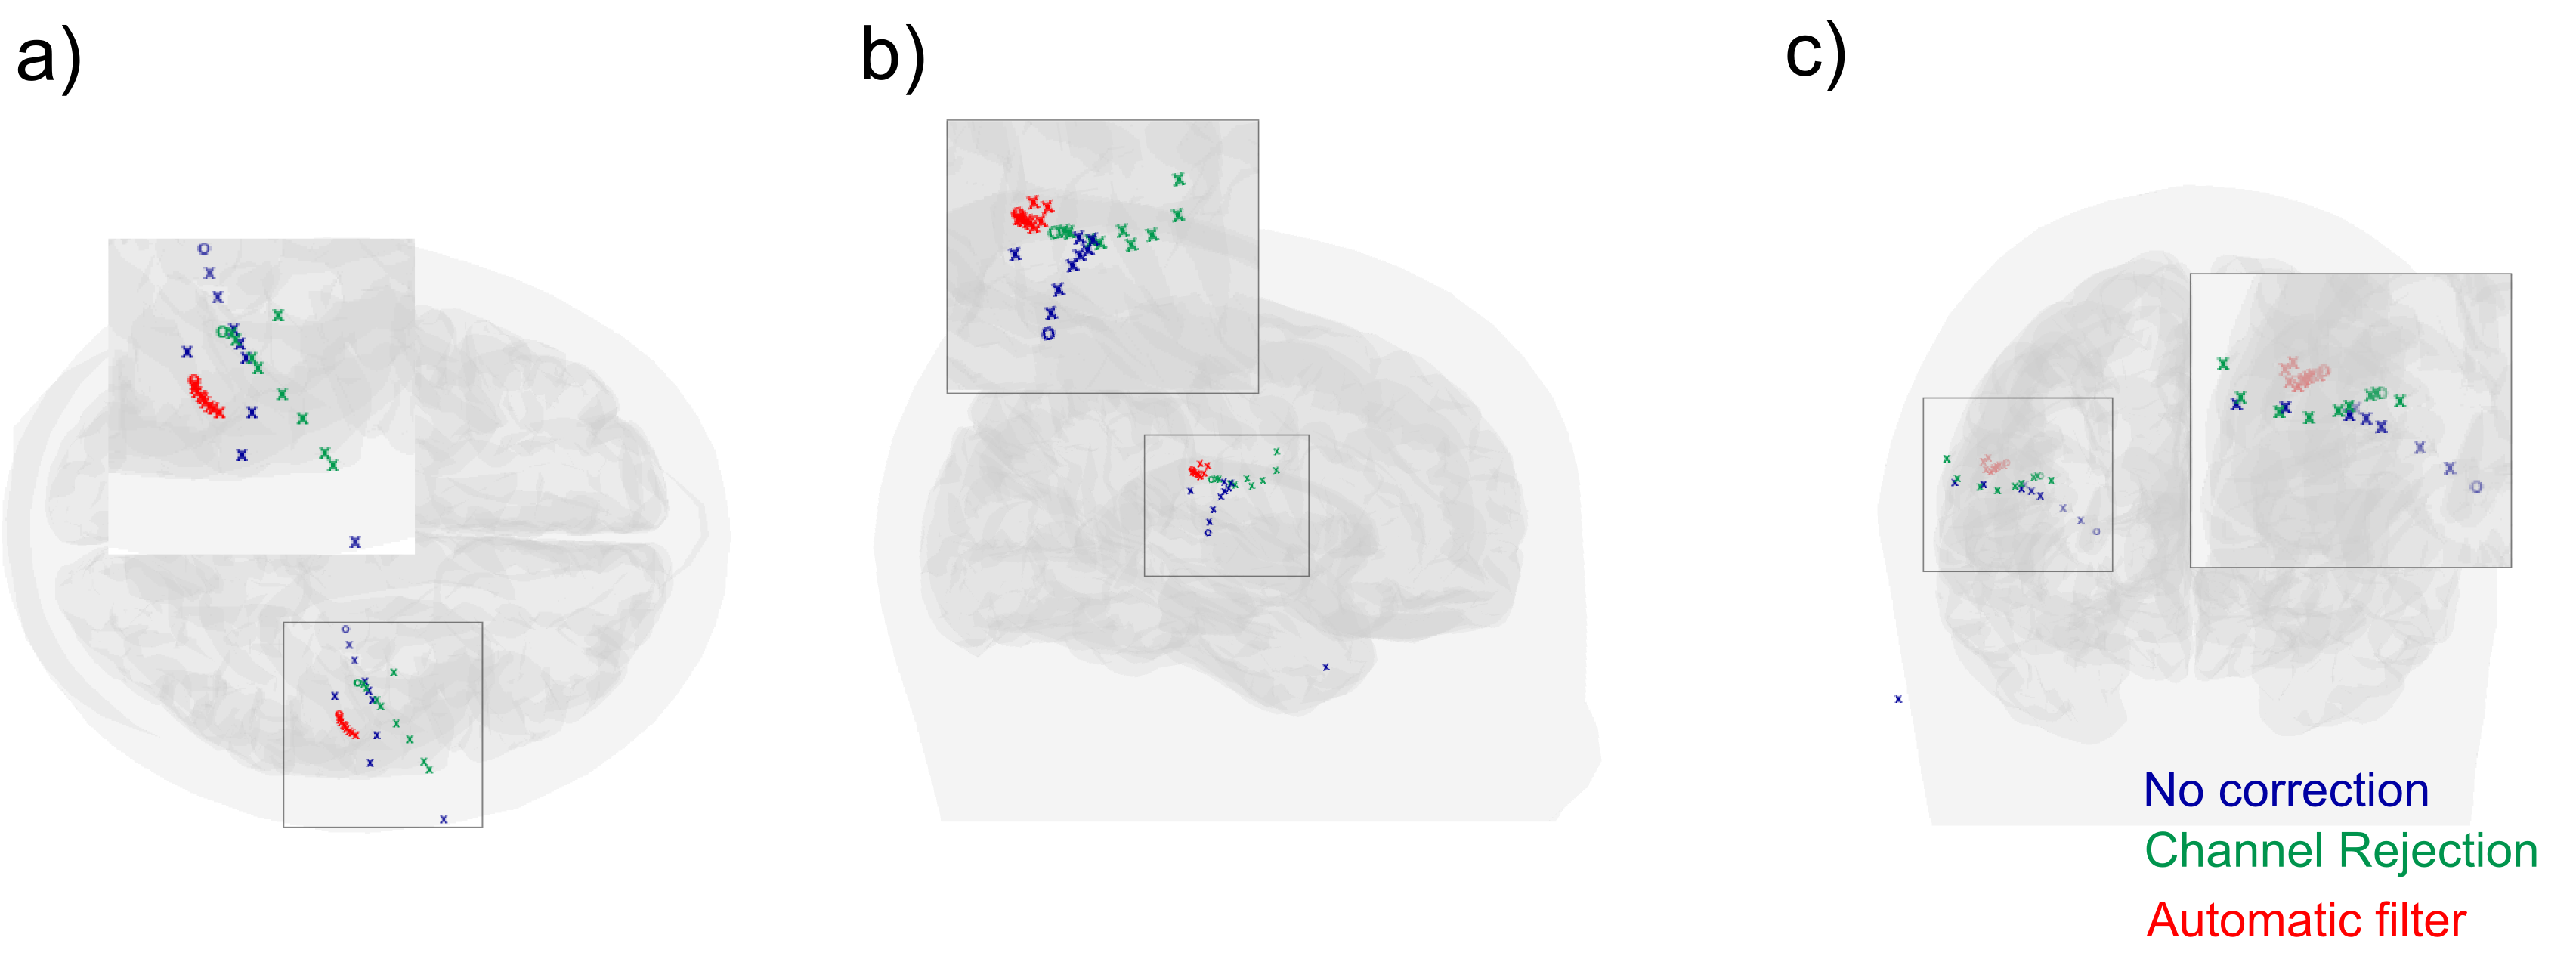
\includegraphics[width=1\textwidth]{Images/fig2-6.png}
\caption{Positions obtained for the consecutive fitted dipoles during the rising phase of an IED. (a) \textit{XY} plane, (b) \textit{XZ} plane and (c) \textit{YZ} plane. Blue, green and red dipoles belong to no-correction, channel rejection and automatic filter procedures. The dipole measured at the onset of the IED is displayed as 'o'.}
\label{fig:2-6}
\end{figure} 

\subsection{Influence of the ASR on dipole localization.}

Metallic artifacts affected MEG signals with different intensity depending on the region of the scalp (see figure \ref{fig:2-3}), which was primarily determined by the nature of the artifact. ASR values, which were defined for the 37-channel region where dipole fitting was performed, are shown in table \ref{tb:2-2}. As ASR increased, ECD fitting of non-corrected MEG data produced more scattered dipoles and therefore a higher dispersion value, as evidenced by the linear regression shown in figure \ref{fig:2-7}.

\begin{figure}[!h]
\centering
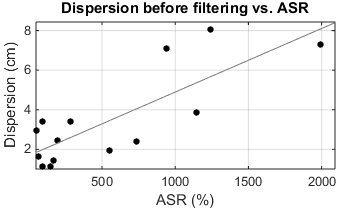
\includegraphics[width=0.7\textwidth]{Images/fig2-7.png}
\caption{Dispersion values versus ASR for the 14 subjects. Linear regression showed a value of r = 0.80 (\textit{p-value} = 0.0005).}
\label{fig:2-7}
\end{figure} 

Two additional regressions were studied to assess the influence of artifact levels on ECD fitting before and after applying the BSS-based automatic reduction of metallic artifacts, as shown in figure \ref{fig:2-8}. Figure \ref{fig:2-8}(a) is a scatterplot of ASR versus the distance between central source position before and after the automatic artifact reduction procedure for all subjects. For small ASR values, distances were lower than 1 cm, but they increased as ASR did. An equivalent analysis was performed for differences in dispersion measures, shown in figure \ref{fig:2-8}(b), and similar results were obtained indicating higher dispersion as ASR increased. Regression lines showed values of r = 0.75 (\textit{p-value} = 0.002) and 0.89 (\textit{p-value} $<$ 0.001), respectively.

\begin{figure}[!h]
\centering
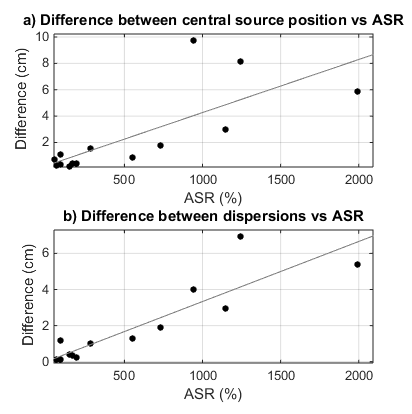
\includegraphics[width=0.8\textwidth]{Images/fig2-8.png}
\caption{(a) Difference between central source position before and after applying automatic filtering procedure versus ASR. Regression line showed a value of r = 0.75 (\textit{p-value} = 0.002). (b) Difference between dispersions versus ASR. Regression line showed a value of r = 0.89 (\textit{p-value} $<$ 0.001).}
\label{fig:2-8}
\end{figure} 

\section{Discussion}

Patients suffering from refractory epilepsy usually have to undergo resective surgery, and this process requires an extensive presurgical evaluation to determine the epileptogenic area and to plan the suitable strategies for neurosurgery, taking into account the functions of nearby areas before the resection. Several studies have determined that MEG interictal epileptiform activity is useful to locate epileptic foci \citep{Shibasaki2007,Enatsu2008,Englot2015}, and although it cannot replace intracranial EEG at the present time \citep{Shibasaki2007}, MEG can often provide additional and useful information mainly because of its whole-head coverage. Even in those cases where intracranial recordings are strictly necessary (generally when the sources are deep), MEG recordings are useful to determine the area where the electrodes will be implanted. This technique has shown superior performance than EEG \citep{Amo2003,Stefan2004,Ramantani2006}.

The standard clinical MEG procedure consists in the inspection of the recordings and the detection of well-defined IEDs so that ECD fitting can be performed to locate an epileptic source. Dealing with metallic artifacts is one of the main drawbacks of the MEG technique because they can affect many subjects \citep{Vrba2002}. For Elekta-Neuromag systems, the tSSS approach has proven to be effective removing metallic interference coming from different sources \citep{Song2009,Kakisaka2012,Jin2013,Wang2013}. As explained before, this technique is not applicable to signals from different MEG systems and the algorithm is not freely available. There are no comparative studies among this technique with other artifact reduction algorithms such as BSS. The analysis of the differences and advantages of these two algorithms in Elekta MEG systems would be an interesting field of study. In an interesting study held by \citep{GonzalezMoreno2014} an SNR analysis was carried out applying tSSS followed by a BSS procedure. The study concluded that SNR increased by 100\% after applying tSSS techniques and an additional 33\%–36\% after applying BSS methods suggesting that not all noise was successfully removed by the tSSS method.

In this study, the effectiveness of an automatic BSS-based artifact reduction procedure algorithm, described in detail and validated in \citep{Migliorelli2015}, was evaluated in patients with refractory focal epilepsy. A comparative analysis of ECD estimation through different usual clinical approaches was performed: using MEG signals without any metallic artifact correction; rejecting highly affected channels; and applying the automatic BSS-based procedure. The resulting dipole locations corresponding to ten well-defined IEDs were analyzed.

Metallic artifacts can be produced by different sources such as dental implants or brackets, cerebral implants such as intracranial electrodes or subdural grids, vagal stimulators, and ventricular bypass valves, among others. Depending on the kind of source, its size and its position, metallic artifacts can affect different areas of the scalp with varying intensity. This variability generates multiple situations in which artifacts can impact on big areas, or appear localized in a specific region with different intensity, usually exceeding the energy of cerebral activity by several orders of magnitude. The BSS-based automatic artifact correction procedure was able to successfully detect independent components associated to metallic activity and allowing an effective reduction of their effects. This methodology also provided an objective measure of the high variability observed in metallic artifacts as quantified by independent component detection: subjects with very focused artifacts (patients 2, 9, 13, and 14) presented fewer components related to metallic artifacts than subjects with artifacts more spread over the head (patients 3, 6, and 12).

Recordings affected by metallic interference produced highly artifacted temporal signals where brain activity appeared completely masked in some electrodes or regions. Detection of interictal epileptiform activity in this scenario may be a challenging task in clinical routine, especially in cases where the artifacted region overlaps the area where IEDs show maximum magnetic activity. As shown in the example in figure \ref{fig:2-3}, metallic interference mainly affected channels in red and was successfully removed from the MEG signal after applying the BSS-based artifact reduction procedure. Although some well-defined IEDs were detected in the artifacted recordings, spike identification became easier after artifact reduction.

Even if well-defined IEDs can be detected in the presence of metallic artifacts, ECD estimation may produce dipoles whose position is outside the brain. It is important to notice that high values of \textit{gof} and low values of \textit{V} do not imply a feasible physiological location, since this two measures only quantify the fitting of real data to the dipolar model. In other words, if measured data correspond to dipolar sources outside the brain, the ECD estimation will be able to fit a dipole with an excellent \textit{gof} and low \textit{V}. That is the main reason why the naive approach of using signals without any kind of artifact correction and even the artifacted channel rejection strategy produced several dipoles located outside the brain. These dipoles were discarded for further analysis, and consequently these two approaches provided fewer dipoles than the automatic artifact reduction. This approach always produced dipoles inside the brain and its dispersion and distance measures were computed using all the ten identified IEDs.

For each subject, all the identified IEDs produced similar magnetoencephalographic activity and exhibited their maximum value at the same area of the scalp, showing a similar dipolar distribution. Under these circumstances, the identified IEDs were expected to be generated by the same internal sources. The dispersion of the location of the fitted dipoles with respect to their average (central source position) was calculated for each subject for the three approaches: naïve, channel rejection, and automatic artifact reduction. As expected, the best results were obtained for the artifact reduction approach. Although more dipoles were obtained inside the brain when performing channel rejection, the corresponding dispersion values did not significantly improve with respect to the naïve approach.

The beginning of epileptiform activity is represented by IED onset, and thus this is the desired point to apply ECD estimation \citep{Bagic2011}. However, the point with the lowest signal-to-noise ratio corresponds to the peak value of a spike. The rising phase of the IED progresses between these two instants and the dipole moves due to the propagation of the epileptiform activity. Observing and characterizing the course of these propagations could be considered a reliable way of assessing the likelihood of the estimated dipoles after the application of different artifact reduction methodologies. Stable dipole trajectories, without abrupt changes of position or direction, are most likely associated with a single cerebral source and can be explained by a single-dipole model \citep{Townsend2008} (Townsend and Ebersole 2008). Following this reasoning, several dipoles, estimated during the rising phase of an IED, are shown in figure \ref{fig:2-6}. Interestingly, the distribution of dipoles exhibited a more stable time course and distribution after automatic artifact correction, whereas dipoles should be discarded for further analysis due to instability in the other two approaches. Stability was measured by the running distance of IED paths for all patients, and results of table \ref{tb:2-2} evidenced significantly reduced distances for the automatic artifact reduction approach. Removing artifacted channels did not produce any improvement in distances and therefore in the stability of the dipole during the rising phase of the IED.

Metallic artifacts can affect recordings with varying energy, projecting on different areas of the scalp. In order to analyze the effect of metallic artifacts on detected IEDs, the relationship between their dispersion and the ASR for artifacted data is shown in figure \ref{fig:2-7}. Results indicated more variability in the location of estimated ECDs of a subject when metallic artifacts were higher, resulting in higher values of dispersion. In this sense, the differences in central source position and dispersion observed before and after applying the BSS-based automatic artifact reduction procedure evidenced that dipole locations changed significantly for high values of ASR, but were not altered when lower levels of artifacts were present (see figure \ref{fig:2-8}). Noticeably, the high dispersion values shown in figure \ref{fig:2-7} corresponded to the highest differences depicted in figure \ref{fig:2-8}, demonstrating that the artifact reduction approach produced a more reliable ECD estimation thanks to reduced levels of metallic artifacts.

Although the results show a significant improvement of the dipole fitting procedure, an additional validation with the actual localization of the epileptic focus would have been useful. However, in this study, no detailed information about surgery or intracranial electrodes data was available. Nevertheless, lower levels of dispersion and distance measures shown by data after applying the artifact reduction procedure suggested an improvement in the stability of the dipolar sources and therefore a more reasonable association with the discharges produced by the epileptic tissue.

Hence, the results encourage the use of such a BSS-based automatic artifact reduction procedure to improve IED detection and realiable ECD fitting in these patients whose MEG recordings are affected by metallic interference, which otherwise would not be suitable for presurgical analysis and would require alternative and possibly more invasive strategies to prepare for resective surgery.

\section{Acknowledgments}

CIBERBBN is an initiative of the Instituto de Salud Carlos III, Spain. This work has been partially supported by the Ministry of Economy and Competitiveness (MINECO), Spain, under contract DPI201459049R and the Ministry of Education, Culture and Sports (MECD) FPU12/05631.